\pgfplotstablegetelem{\thepart}{[index]\columnIndex}\of{\cronograma}
\part{\pgfplotsretval}
\label{part:\thepart}
\frame{\partpage}


\begin{frame}[t]{Exemplos de criação de classe}
	
	\fontsize{14pt}{15}\selectfont{
		
		...continuando a partir da aula passada sobre \gls{poo}.
		
	}\par
	\vspace{1em}
	
	
\end{frame}







\begin{frame}[t]{Herança em classes}
	
	\fontsize{14pt}{15}\selectfont{
		
		Permite que uma classe seja definida com base em classe já existente. Dizemos que essa nova classe herda características da classe original.
		
	}\par
	\vspace{1em}
	
	\fontsize{12pt}{15}\selectfont{
		\begin{itemize}%[<+->] 
			
			\item Na terminologia Python a classe original é chamada de Classe Base, Classe Mãe ou Superclasse (Base, Parent ou Super Class) enquanto que a nova é chamada de Sub Classe ou Classe Filha (Sub ou Child Class).
			
			\item A subclasse pode especializar a classe principal ou mesmo estendê-la com novos métodos e atributos.
			
		\end{itemize}
	}\par
	\vspace{1em}
	
\end{frame}





\begin{frame}[t]{Herança em classes}
	
	\fontsize{14pt}{15}\selectfont{
		
		Uma classe não precisa necessariamente ter um método construtor. Podemos ter uma classe apenas com métodos, sem atributos. Nesse caso, o nome da classe é usado sem parâmetros para a chamada das funções.
		
	}\par
	\vspace{1em}
	
	\fontsize{14pt}{25}\selectfont{
		\begin{beamercolorbox}[wd=\textwidth]{warning}
			class Produto:\\		
			
			\hspace{1em}def imprime\_nome(nome):\\
			\hspace{2em}print(nome)\\
			\vspace{1em}
			Produto.imprime\_nome('Arroz')
			
		\end{beamercolorbox}
		
	}\par
	\vspace{1em}
	
\end{frame}



\begin{frame}[t]{Herança em classe}	
	
	\lstinputlisting[style=CBruno,caption=Herança da classe Produto]{outros/codigos/python/exemplos-de-aulas/src/codigo_004_classe_produto_critico.py}
	
	
	*obs: \textbf{class ProdutoCritico(Produto)} é uma classe derivada de Produto: indica que \textbf{ProdutoCritico} é uma subclasse da classe \textbf{Produto}.
	
\end{frame}

\begin{frame}[t]{Pytest}
	
	\vspace{-1em}
	\lstinputlisting[style=CBruno,caption=Cobertura de testes da classe Produto Crítico]{outros/codigos/python/exemplos-de-aulas/tests/test_codigo_004_classe_produto_critico.py}
	
	
\end{frame}



\begin{frame}[t]{Pytest}
	
	
	\vspace{1em}
	\centering
	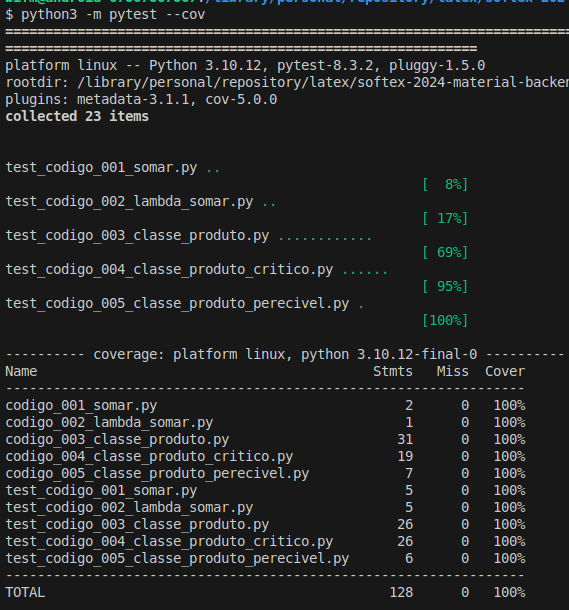
\includegraphics[scale=0.3]{imagens/fig-result-test-produto-critico.png}
	
\end{frame}








\begin{frame}[t]{Exercícios}
	
	\fontsize{12pt}{19}\selectfont{
		Escreva o algoritmo e programa. Use Herança de \gls{poo} para resolver.
		\begin{itemize}%[<+->]
			
			\item \glsfirst{exercicio_018}: \glsdesc{exercicio_018}
			
			\vspace{1em}
			\centering
			
\includegraphics[scale=0.13]{imagens/fig-atencao-pessoas-estudando.png}
			
			%			\item \glsfirst{exercicio_014}: \glsdesc{exercicio_014}
			
		\end{itemize}
	}\par
	\vspace{1em}
	
	
	
\end{frame}





